
\documentclass[si.tex]{subfiles}

\begin{document}

\subsubsection{Theoretical Guarantee}

Here, we show how our identifiability guarantees apply for two-alternative forced-choice (2AFC) tasks.
In such experiments, subjects are typically presented with two stimuli in the same trial, and asked to judge which one is larger.

We assume the following generative model of a single trial in the 2AFC task:
\begin{enumerate}
    \item Encode $\theta_1, \theta_2$ independently, according to the sensory noise levels $\sigma_1, \sigma_2$ at which each of them is presented: $m_1 = F(\theta_1) + \sigma_1 \epsilon_1$, $m_2 = F(\theta_2) + \sigma_2 \epsilon_2$ where $\epsilon_1, \epsilon_2 \sim N(0,1)$ independent.
    \item Decode $\widehat{\theta_1}$ from $m_1$, $\widehat{\theta_2}$ from $m_2$.
    \item Respond based on which of these is larger. There may be a nonzero lapse rate, determining 
\end{enumerate}
This is essentially the model assumed by \citet{Girshick2011CardinalRV, Stocker2005}.



We first point out that, except for the role of motor noise, forced choice provides no information beyond that contained in response distributions. This because one can simulate a 2AFC task by encoding and decoding the two stimuli separately and compare the response distributions.
We now investigate to what extent 2AFC response distributions might provide \emph{the same} information as response distributions, and allow recoverability.
2AFC response distributions where both stimuli are subjected to the same sensory noise recover exactly the encoding, but provide no information about prior and loss function, due to (\ref{eq:comparison-encodings-cumulative}).
We now investigate the more general setting of 2AFC Response distributions when the two stimuli are subjected to different amounts of noise.
These can be expected to provide information about the \emph{relative bias} between two conditions.
Intuitively, comparing this across multiple conditions should enable recovering the bias.
Formally, we obtain a guarantee analogous to Theorem 2, though three levels of sensory noise are required:
%
%
%In the limit $\sigma_1, \sigma_2, \sigma_3 \rightarrow 0$, models outside of $\Omega$ can be fully identified from the full 2AFC response distributions at 3 levels of sensory noise $\sigma_1, \sigma_2, \sigma_3$ when $0 < C_1 < \frac{\sigma_1}{\sigma_2}, \frac{\sigma_2}{\sigma_3} < C_2 < \infty$.
%
%
\begin{thm}
%
There is a function $\Phi$ mapping 2AFC response distributions to $\tilde{M} \in \mathfrak{M}$ such that the following holds.
Assume $0 < \sigma_1^2 < \sigma_2^2 < \sigma_3^2$ are three sensory noise variances.
Assume the response distribution is derived at noise levels $\sigma_1^2, \sigma_2^2, \sigma_3^2$ and lapse rate $\lambda > 0$ from the ground-truth model $M = \langle F', \Prior,p \rangle \in \mathfrak{M}$.
Then for the model
\begin{equation}
\tilde{M} = \langle \tilde{F}', \tilde{\Prior},\tilde{q}\rangle \in \mathfrak{M}
\end{equation}
output by $\Phi$, we have -- provided $M \not\in \Omega$ -- the following for all $\theta$
\begin{align*}
    \widehat{F}(\theta) &= F(\theta) + \mathcal{O}(\sigma_1^2) &
    \tilde{\Prior}(\theta) &= \Prior(\theta) + \mathcal{O}(\sigma_1^2) &
    \tilde{q} &= p  \text{ for $\sigma_1^2$ small}
\end{align*}
in the limit where $\sigma_1, \sigma_2, \sigma_3 \rightarrow 0$, provided: 
\begin{align*}
0 < C_1 < \frac{\sigma_1}{\sigma_2}, \frac{\sigma_2}{\sigma_3} < C_2 < 1 < \infty     
\end{align*}
for some $C_1, C_2, C_3, C_4$, and $\sigma_2-\sigma_1 \neq \sigma_3-\sigma_2$.
Constants in the $\mathcal{O}(\cdot)$ expressions depend on $C_1, C_2, C_3, C_4$, and on the regularity of $F$ and $\Prior$ and their derivatives, but not on $\theta$.
%Membership in $\Omega$ can be explicitly verified. For any model in $\Omega$, there are at most five models indistinguishable from it, and they can be explicitly enumerated.

\end{thm}

\begin{proof}
As in the proof of Theorem 2, we introduce a parameter $t$ such that $\sigma_1, \sigma_2, \sigma_3$ are constant multiplies of $t$ as $t\rightarrow 0$.
First, we note that the lapse rate can be identified, when $t$ is small, from the response distribution when $\theta_1$ and $\theta_2$ are very far away. 
Second, $F$ and $\sigma_1, \sigma_2, \sigma_3$ can already be inferred from response distributions under equal sensory noise by Theorem~\ref{lemma:f-exact}.
We now specifically consider a pair of sensory noise magnitudes, say, $\sigma_1, \sigma_2$.
Assume that $\theta_1$ and $\theta_2$ are perceived at sensory noise magnitudes $\sigma_1, \sigma_2$, respectively.
Then, for the respective decoded estimates $\widehat{\theta_1}$, $\widehat{\theta_2}$:
\begin{align*}
    \mathbb{P}(\widehat{\theta_1} < \widehat{\theta_2}) =& \mathbb{P}\left(f_1(F(\theta_1)+\sigma_1 \epsilon_1) < f_2(F(\theta_2)+\sigma_2 \epsilon_2)\right) \\
    =& \mathbb{P}\left(F(\theta_1)+\sigma_1 \epsilon_1 < f_1^{-1}(f_2(F(\theta_2)+\sigma_2 \epsilon_2))\right) 
\end{align*}
where $f_1, f_2$ are the two decoding functions (Definition~\ref{def:decoding-funct}) mapping $F^{-1}(m)$ to the estimate $\widehat{\theta}$, under noise magnitudes $\sigma_1, \sigma_2$, respectively.
This permits recovering the function
\begin{align*}
    f_1^{-1} \circ f_2 : \theta \mapsto f_1^{-1}(f_2(\theta))
\end{align*}
In the low-noise regime, writing $\sigma_1 = at$ and $\sigma_2 = bt$, we can write
\begin{align*}
    f_1(\theta) = \theta + at\mathcal{C}_{dec}(\theta)+ a^2t^2 \mathcal{D}_{dec}(\theta) + O(t^3) \\
    f_2(\theta) = \theta + bt\mathcal{C}_{dec}(\theta)+ b^2t^2 \mathcal{D}_{dec}(\theta) + O(t^3) 
\end{align*}
where $\mathcal{C}_{dec}$ and $\mathcal{D}_{dec}$ as per Eq.~\ref{eq:expansion-f}. 
We now aim to show the following:
\begin{equation}\label{eq:f1-f2-composed}
f_1^{-1}(f_2(\theta)) = \theta + (b-a)t\,\mathcal{C}_{dec}(\theta) + t^2\Bigl[(b^2-a^2)\mathcal{D}_{dec}(\theta)-a(b-a)\mathcal{C}_{dec}(\theta)\mathcal{C}_{dec}'(\theta)\Bigr] + O(t^3).
\end{equation}
Now, comparing the expression for $f_1^{-1}(f_2(\theta))$ between two different  noise level pairs (e.g. $\sigma_1$ and $\sigma_2$ vs $\sigma_2$ and $\sigma_3$) permits identifying $\mathcal{C}_{dec}$ and $\mathcal{D}_{dec}$ up to error $O(t)$ each.
This, in turn, permits identifying the full model as long as it is not in $\Omega$.
This is because two models have identical $F, \mathcal{C}_{dec}, \mathcal{D}_{dec}$ if and only they have identical $F, \mathcal{C}, \mathcal{D}$ (see Eq.~\ref{eq:dm-decomposition} for $\mathcal{D}$).


It now remains to show (\ref{eq:f1-f2-composed}).
We are given the functions
\begin{align}
f_1(x) &= x + at\,\mathcal{C}_{dec}(x) + a^2t^2 \mathcal{D}_{dec}(x) + O(t^3), \label{f1}\\[1mm]
f_2(x) &= x + bt\,\mathcal{C}_{dec}(x) + b^2t^2 \mathcal{D}_{dec}(x) + O(t^3), \label{f2}
\end{align}
where \( t > 0 \) is small. Our goal is to express 
\[
f_1^{-1}(f_2(\theta))
\]
in terms of \( \mathcal{C}_{dec}(\theta) \), \( \mathcal{D}_{dec}(\theta) \), and derivatives of \( \mathcal{C}_{dec}(\theta) \).
Assume that the inverse has the expansion
\[
x = f_1^{-1}(f_2(\theta)) = \theta + \epsilon_1 t + \epsilon_2 t^2 + O(t^3),
\]
with unknown coefficients \(\epsilon_1\) and \(\epsilon_2\) to be determined.
Since
\[
f_1(x) = x + at\,\mathcal{C}_{dec}(x) + a^2t^2\mathcal{D}_{dec}(x) + O(t^3),
\]
substitute \( x = \theta + \epsilon_1t + \epsilon_2t^2 \):
\[
f_1(\theta+\epsilon_1t+\epsilon_2t^2)
=\theta+\epsilon_1t+\epsilon_2t^2 + at\,\mathcal{C}_{dec}(\theta+\epsilon_1t+\epsilon_2t^2) + a^2t^2\mathcal{D}_{dec}(\theta+\epsilon_1t+\epsilon_2t^2) + O(t^3).
\]
We now expand \( \mathcal{C}_{dec}(\theta+\epsilon_1t+\epsilon_2t^2) \) using Taylor's theorem:
\[
\mathcal{C}_{dec}(\theta+\epsilon_1t+\epsilon_2t^2)
= \mathcal{C}_{dec}(\theta) + \mathcal{C}_{dec}'(\theta)(\epsilon_1t+\epsilon_2t^2) + \frac{1}{2}\mathcal{C}_{dec}''(\theta)(\epsilon_1t)^2 + O(t^3).
\]
Retaining terms up to \( t^2 \), we have
\[
\mathcal{C}_{dec}(\theta+\epsilon_1t+\epsilon_2t^2)
= \mathcal{C}_{dec}(\theta) + \epsilon_1t\,\mathcal{C}_{dec}'(\theta) + O(t^2).
\]
Similarly, for \( \mathcal{D}_{dec}(\theta+\epsilon_1t+\epsilon_2t^2) \) we need only
\[
\mathcal{D}_{dec}(\theta+\epsilon_1t+\epsilon_2t^2)
= \mathcal{D}_{dec}(\theta)+O(t).
\]
Substituting these into the expansion for \( f_1(x) \) yields:
\begin{align*}
f_1(\theta+\epsilon_1t+\epsilon_2t^2)
&= \theta+\epsilon_1t+\epsilon_2t^2 + at\Bigl(\mathcal{C}_{dec}(\theta)+\epsilon_1t\,\mathcal{C}_{dec}'(\theta)\Bigr) + a^2t^2\mathcal{D}_{dec}(\theta) + O(t^3)\\[1mm]
&= \theta+\epsilon_1t+\epsilon_2t^2 + at\,\mathcal{C}_{dec}(\theta) + a\epsilon_1t^2\,\mathcal{C}_{dec}'(\theta) + a^2t^2\mathcal{D}_{dec}(\theta) + O(t^3).
\end{align*}
Simultaneously, from \eqref{f2}, we have
\[
f_2(\theta) = \theta + bt\,\mathcal{C}_{dec}(\theta) + b^2t^2\mathcal{D}_{dec}(\theta) + O(t^3).
\]
Since \( f_1(x) = f_2(\theta) \), we equate coefficients of corresponding powers of \( t \).
First, at order \( t^0 \), we have $\theta=\theta$.
Second, at order \( t^1 \):
\[
\epsilon_1 + a\,\mathcal{C}_{dec}(\theta) = b\,\mathcal{C}_{dec}(\theta).
\]
Thus, we obtain:
\[
\epsilon_1 = (b - a)\mathcal{C}_{dec}(\theta).
\]
Third, at order \( t^2 \):
\[
\epsilon_2 + a\epsilon_1\,\mathcal{C}_{dec}'(\theta) + a^2\mathcal{D}_{dec}(\theta) = b^2\mathcal{D}_{dec}(\theta).
\]
Substitute \(\epsilon_1 = (b-a)\mathcal{C}_{dec}(\theta)\) to get:
\[
\epsilon_2 + a(b-a)\mathcal{C}_{dec}(\theta)\mathcal{C}_{dec}'(\theta) + a^2\mathcal{D}_{dec}(\theta) = b^2\mathcal{D}_{dec}(\theta).
\]
Thus,
\[
\epsilon_2 = b^2\mathcal{D}_{dec}(\theta) - a^2\mathcal{D}_{dec}(\theta) - a(b-a)\mathcal{C}_{dec}(\theta)\mathcal{C}_{dec}'(\theta),
\]
or equivalently,
\[
\epsilon_2 = (b^2-a^2)\mathcal{D}_{dec}(\theta) - a(b-a)\mathcal{C}_{dec}(\theta)\mathcal{C}_{dec}'(\theta).
\]
Substituting the values of \(\epsilon_1\) and \(\epsilon_2\) into the expansion for \( x \) gives:
\[
f_1^{-1}(f_2(\theta)) = \theta + (b-a)t\,\mathcal{C}_{dec}(\theta) + t^2\Bigl[(b^2-a^2)\mathcal{D}_{dec}(\theta)-a(b-a)\mathcal{C}_{dec}(\theta)\mathcal{C}_{dec}'(\theta)\Bigr] + O(t^3).
\]
    \end{proof}



\subsubsection{Simulation}\label{sec:2afc-experiment}


\paragraph*{Implementation}
We focus on circular stimulus spaces.
We start from the likelihoods $P(m_1|\theta_1)$, $P(m_2|\theta_2)$, and the derived estimates $\widehat{\theta}_1$, $\widehat{\theta}_2$.
The generative model for a response stating that ``$\theta_1 > \theta_2$'' has the likelihood:
\begin{align*}
    P(response=1|\theta_1, \theta_2) = \int_{\mathcal{X} \times \mathcal{X}} \widehat{P}(\widehat{\theta}_1=s|\theta_1) \widehat{P}(\widehat{\theta}_2=t|\theta_2) 1_{\sin(s-t) > 0} d(s,t)
\end{align*}
Recall that the implementation of \citet{hahn2024unifying} discretizes the stimulus space via a regularly-spaced grid $x_1, \dots, x_N$; it is thus necessary to define $\widehat{P}(\widehat{\theta}_1=x_s|\theta_1)$ for points $x_s$ on the grid.
We define von Mises kernels ($k=1,2; i = 1, \dots, N$) and normalize these:
\begin{equation}
    \phi_{i,k}(j) = \frac{\exp(\gamma \cdot \cos(\widehat{\theta}_{k,i} - x_j))}{\sum_s \exp(\gamma \cdot \cos(\widehat{\theta}_{k,i} - x_s))}
\end{equation}
where we choose $\gamma = 500$ to make the kernels very narrow, and use these to project the distributions $P(\widehat{\theta}_k|\theta_k)$ onto the grid:
\begin{equation}
    \widehat{P}(\widehat{\theta}_k=x_j|\theta_k) \propto \sum_{s=1}^N \phi_{s,k}(j) P(m_k = x_s|\theta_k)
\end{equation}
We then define
\begin{align*}
    P(response=1|\theta_1, \theta_2) = \sum_{s,t : \sin(x_s-x_t) > 0} \widehat{P}(\widehat{\theta}_1=x_s|\theta_1) \widehat{P}(\widehat{\theta}_2=x_t|\theta_2) + \frac{1}{2} \sum_{s} \widehat{P}(\widehat{\theta}_1=x_s|\theta_1) \widehat{P}(\widehat{\theta}_2=x_s|\theta_2)
\end{align*}
For simplicity, our simulations assume a zero lapse rate.

\paragraph*{Experiment}

We generate uniformly distributed $\theta_1$, and then choose $\theta_2$ uniformly at a distance of $\leq 40^\circ$ when viewing the full sensory space as a full 360$^\circ$ circle ($\cos(\theta_1-\theta_2) \gtrapprox 0.76$).
We note that, in principle, staircase procedures could be used to optimize the selection of stimuli in an experiment. However, such an adaptive procedure is substantially more complex to implement than the simple estimation paradigm.
We compared two setups: one where the reference is provided at the same noise as the lowest-noise test condition, and one where the the reference is encoded without any noise. Results show that, while the encoding is fitted in both cases, only the latter setup permits identifying prior and loss function (Figure~\ref{fig:2afc}). Overall, this result suggests 2AFC can be used in principle to identify models, as it theoretically provides the same information as the estimation paradigm. However, at a finite number of trials, at least without adaptive choice of stimuli, the simple estimation procedure is likely to be more efficient.



\begin{figure}


\begin{comment}

python3 Run_2AFC_Synthetic_FreePrior_CosineLoss_OnSim_RUNALL.py
python3 Run_2AFC_Synthetic_FreePrior_CosineLoss_OnSim_CleanRef_RUNALL.py

python3 Run_2AFC_Synthetic_FreePrior_CosineLoss_OnSim_VIZ.py 2 0 10.0 180 Simulate_2AFC_Synthetic_Parameterized_OtherNoiseLevels_Grid_VarySize_WithKL.py_180_2_T5_S80.0_2345_40000_STEEPPERIODIC_STEEPPERIODIC.txt
python3 Run_2AFC_Synthetic_FreePrior_CosineLoss_OnSim_CleanRef_VIZ.py 2 0 10.0 180 Simulate_2AFC_Synthetic_Parameterized_OtherNoiseLevels_Grid_VarySize_WithKL_CleanRef.py_180_2_T9_S80.0_2345_40000_STEEPPERIODIC_STEEPPERIODIC.txt
#python3 Run_2AFC_Synthetic_FreePrior_CosineLoss_OnSim_VIZ.py 8 0 10.0 180 Simulate_2AFC_Synthetic_Parameterized_OtherNoiseLevels_Grid_VarySize_WithKL.py_180_8_T5_S80.0_2345_40000_STEEPPERIODIC_STEEPPERIODIC.txt
#python3 Run_2AFC_Synthetic_FreePrior_CosineLoss_OnSim_CleanRef_VIZ.py 8 0 10.0 180 Simulate_2AFC_Synthetic_Parameterized_OtherNoiseLevels_Grid_VarySize_WithKL_CleanRef.py_180_8_T9_S80.0_2345_40000_STEEPPERIODIC_STEEPPERIODIC.txt


python3 evaluateCrossValidationResults_Synthetic_Gardelle_2AFC.py  Simulate_2AFC_Synthetic_Parameterized_OtherNoiseLevels_Grid_VarySize_WithKL.py_180_2_T5_S80.0_2345_40000_STEEPPERIODIC_STEEPPERIODIC.txt
python3 evaluateCrossValidationResults_Synthetic_Gardelle_2AFC_CleanRef.py  Simulate_2AFC_Synthetic_Parameterized_OtherNoiseLevels_Grid_VarySize_WithKL_CleanRef.py_180_2_T9_S80.0_2345_40000_STEEPPERIODIC_STEEPPERIODIC.txt
#python3 evaluateCrossValidationResults_Synthetic_Gardelle_2AFC.py  Simulate_2AFC_Synthetic_Parameterized_OtherNoiseLevels_Grid_VarySize_WithKL.py_180_8_T5_S80.0_2345_40000_STEEPPERIODIC_STEEPPERIODIC.txt
#python3 evaluateCrossValidationResults_Synthetic_Gardelle_2AFC_CleanRef.py  Simulate_2AFC_Synthetic_Parameterized_OtherNoiseLevels_Grid_VarySize_WithKL_CleanRef.py_180_8_T9_S80.0_2345_40000_STEEPPERIODIC_STEEPPERIODIC.txt

\end{comment}



\centering
%\textbf{Example 1: $p=2$}

Original Model ($p=2$)

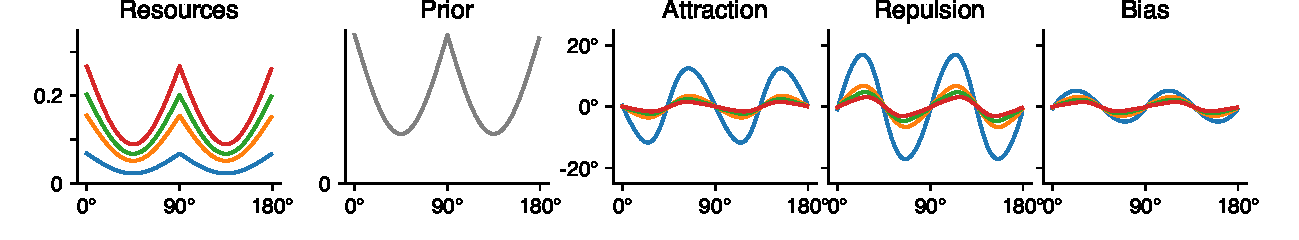
\includegraphics[width=0.65\textwidth]{figures/CounterfactualModel_VIZ.py_2345_STEEPPERIODIC_STEEPPERIODIC_2_0_10.0_180.pdf}

\ \ 

\ \ 


Fitted (Reference: Low-Noise Condition)

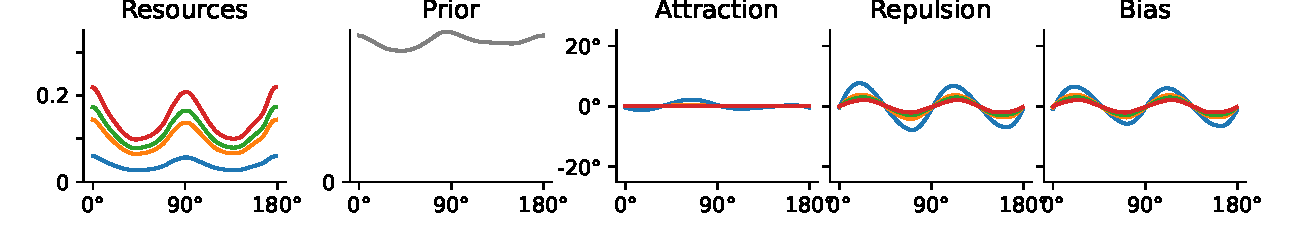
\includegraphics[width=0.65\textwidth]{figures/Run_2AFC_Synthetic_FreePrior_CosineLoss_OnSim_VIZ.py_Simulate_2AFC_Synthetic_Parameterized_OtherNoiseLevels_Grid_VarySize_WithKL.py_180_2_T5_S80.0_2345_40000_STEEPPERIODIC_STEEPPERIODIC.txt_2_0_10.0_180.pdf}
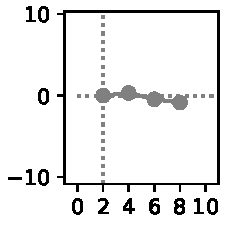
\includegraphics[width=0.15\textwidth]{figures/evaluateCrossValidationResults_Synthetic_Gardelle_2AFC.py_Simulate_2AFC_Synthetic_Parameterized_OtherNoiseLevels_Grid_VarySize_WithKL.py_180_2_T5_S80.0_2345_40000_STEEPPERIODIC_STEEPPERIODIC.txt_RelativeLF.pdf}

\ \ 

\ \ 

Fitted (Reference: Fully Noise-Free)

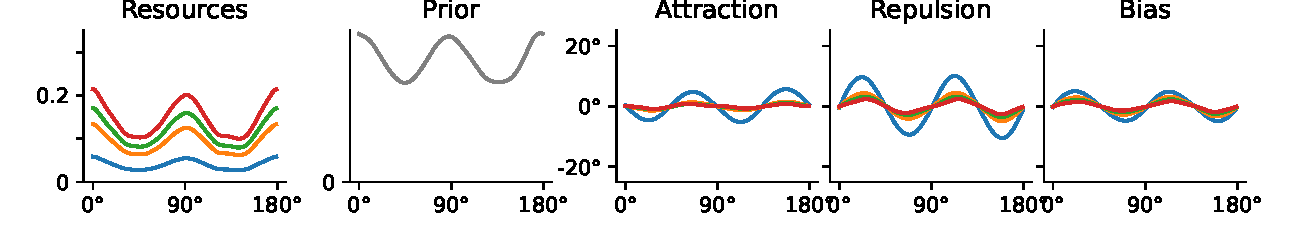
\includegraphics[width=0.65\textwidth]{figures/Run_2AFC_Synthetic_FreePrior_CosineLoss_OnSim_CleanRef_VIZ.py_Simulate_2AFC_Synthetic_Parameterized_OtherNoiseLevels_Grid_VarySize_WithKL_CleanRef.py_180_2_T9_S80.0_2345_40000_STEEPPERIODIC_STEEPPERIODIC.txt_2_0_10.0_180.pdf}
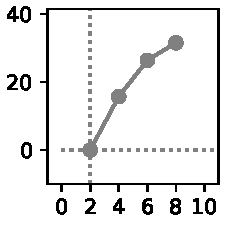
\includegraphics[width=0.15\textwidth]{figures/evaluateCrossValidationResults_Synthetic_Gardelle_2AFC_CleanRef.py_Simulate_2AFC_Synthetic_Parameterized_OtherNoiseLevels_Grid_VarySize_WithKL_CleanRef.py_180_2_T9_S80.0_2345_40000_STEEPPERIODIC_STEEPPERIODIC.txt_RelativeLF.pdf}



\caption{Results from simulated 2AFC paradigm, at N=40K trials (Section~\ref{sec:2afc-experiment}). We considered the cases where the reference either has the same noise level as the least-noisy test condition or is noise-free. Fits were only obtained at $p \geq 2$ due to numerical challenges at lower $p$. The encoding is generally recovered well; the prior and the loss function are recovered more accurately when the reference is noise-free.}\label{fig:2afc}

\end{figure}



\end{document}
